\documentclass{article}
\usepackage{graphicx}
\usepackage{natbib}
\usepackage{amsmath}
\usepackage{amssymb}
\usepackage{booktabs}
\usepackage{array}
\usepackage[margin=1in]{geometry}
\usepackage{hyperref}
\usepackage{xcolor}
\usepackage{changepage}

\definecolor{notecolor}{rgb}{0.5,0.5,0.5}
\newcommand{\draftnote}[1]{\textit{\textcolor{notecolor}{[#1]}}}

\title{Aligning Incentives in the NBA Draft:\\
       A Multi-Agent Simulation of Mechanism Design}
\author{Grant Valentine \and Kartik Dhinakaran}
\date{May 2026}

\begin{document}

\maketitle
\tableofcontents
\newpage

% ============================================================
%  Section 0: Preface
% ============================================================

\section*{Preface}
\addcontentsline{toc}{section}{Preface}

This project was completed jointly by Grant Valentine and Kartik Dhinakaran.
Both authors read through the full literature.
Kartik took primary responsibility for synthesizing the literature review,
with a focus on the empirical and theoretical literature on tanking incentives
\citep{taylor2002, schmidt2024, lenten2016}.
Grant took primary responsibility for the papers on alternative draft
mechanisms \citep{banchio2020, kazachkov2020, highley2026}.
Grant wrote the formal model.
Kartik wrote the introduction and background section.
Both authors contributed to the simulation code: Grant designed the overall
structure and experimental framework, and Kartik implemented the
mechanism-specific logic for each draft system under study.
Writing and analysis were reviewed by both authors throughout.

No external collaborators contributed to this submission beyond high-level
discussion with other students in the course.

% ============================================================
%  Section 1: Research Question & Core Framing
% ============================================================

\section{Research Question \& Core Framing}

Deliberately losing games to improve future draft position, colloquially known
as tanking, has been a persistent problem in professional sports league design
for decades.
The incentive is not subtle: in 1983, the Houston Rockets deliberately
underperformed late in the season to secure the first overall pick in the
following year's draft, ultimately selecting future Hall-of-Famer Hakeem
Olajuwon.
The NBA responded by restructuring the draft lottery, and has done so again in
1990, 2019, and 2026.
Each reform has failed to resolve the underlying problem.
Tanking remains one of the most maligned phenomena in professional basketball,
criticized by fans, analysts, and the league office alike.

This paper asks: to what degree can differing mechanism designs of the NBA
draft influence the incentive for teams to tank while maintaining league-wide
competitive balance?

The central tension is straightforward.
The NBA draft lottery uses reverse-order weighting to promote competitive
balance, a ``rubber band'' effect designed to steer top incoming talent toward
the weakest franchises.
But this structure creates a well-documented adverse incentive: teams near the
bottom of the standings may find it individually rational to lose games
deliberately in order to improve their lottery odds, particularly when the
incoming draft class contains players with asymmetric superstar potential.
The worse a team finishes, the better its expected draft position.
Winning, in this context, can be a mistake.

From an algorithmic game theory perspective, tanking is structurally a
prisoner's dilemma.
A single team that tanks may improve its own long-run competitive outlook, but
when enough teams tank simultaneously, the benefit to any individual team
washes out while the overall quality of league play degrades.
The end-of-season landscape in recent NBA seasons has become increasingly
bifurcated: teams are either competing for playoff seeding or deliberately
losing to improve draft position, with little in between.
The question is whether any mechanism design can resolve this tension
structurally, or whether the impossibility result of \citet{banchio2020}
forecloses the possibility of a clean solution, leaving any viable mechanism
as a tradeoff rather than a fix.

We examine five mechanisms against this tension: the current NBA lottery
(post-2019 reform), the bilevel ranking system proposed by
\citet{kazachkov2020}, the Carry-Over Lottery Allocation (COLA) framework of
\citet{highley2026}, a weighted-loss mechanism that applies a time-decaying
score to each game result, and a proposed NBA redesign in which the three
worst teams receive \emph{fewer} lottery balls than the teams just above them.
We evaluate each through a combination of formal analysis and a multi-agent
simulation in which teams are represented by agents that develop strategies
endogenously, rather than following hardcoded rules.
This approach lets us test how each mechanism performs against adaptive,
strategically sophisticated agents rather than fixed behavioral assumptions.

\begin{table}[h]
\centering
\renewcommand{\arraystretch}{1.3}
\begin{tabular}{p{3.2cm} p{4.2cm} p{5.0cm}}
\toprule
\textbf{Name} & \textbf{Proposer} & \textbf{Key Idea} \\
\midrule
Current NBA lottery &
NBA (2019 reform) &
Reverse-standings weights; top-3 each at 14\% \\
Bilevel ranking &
\citet{kazachkov2020} &
Draft order locked at preset mid-season breakpoint \\
COLA &
\citet{highley2026} &
Equal per-season tickets; persistent losers accumulate carryover advantage \\
Weighted loss &
This paper &
Each loss counts, weighted by exponential decay; early losses matter more \\
NBA ``3-2-1'' proposal &
NBA (proposed) &
Bottom~3 teams receive \emph{fewer} balls than the tier above them \\
\bottomrule
\end{tabular}
\caption{Five mechanisms evaluated in this paper.}
\label{tab:overview}
\end{table}

To evaluate these mechanisms empirically we build a large-scale multi-agent
simulation: 30 teams, 82 games per season, 50 seasons per run, producing
over 123{,}000 game outcomes and 12{,}000 agent decisions per experimental
condition.
Two agent types provide complementary perspectives: a \emph{rational agent}
that maximizes expected utility analytically via normal-approximation
probability estimates, and an \emph{LLM agent} powered by
\texttt{claude-haiku-4-5} that reasons qualitatively about the same
decision.
Running both types across all five mechanisms yields a dataset rich enough
to test each mechanism's theoretical properties against adaptive strategic
behavior.

% ============================================================
%  Section 2: Introduction & Background
% ============================================================

\section{Introduction \& Background}

The NBA is a league consisting of 30 teams, 16 of which make the playoffs each
year.
The remaining 14 non-playoff teams enter a weighted lottery of ping pong balls,
with the composition of balls equivalent to the allotted odds each team has to
pick in the top 4 slots.
From there, slots 5 through 14 are allocated by reverse regular-season record;
slots 15 through 30 occur in the same manner for playoff teams.
The worst pick the team with the worst record could receive is \#5.

This structure has evolved and been re-weighted on multiple occasions by the
NBA:
\begin{itemize}
    \item \textbf{1985:} All 7 non-playoff teams had identical odds at the
    \#1 pick. There is a conspiracy theory surrounding this first lottery
    called the ``frozen envelope'' theory: that Commissioner David Stern, a
    New Yorker, had frozen the NY Knicks envelope so that he would recognize
    it and ensure they selected future Hall of Famer Patrick Ewing.
    \item \textbf{1990:} Weighted the odds by reverse standings for the first
    time; the worst team had a 16.7\% chance at the \#1 pick.
    \item \textbf{1994:} Tweaked so that the worst team has a 25\% chance at
    the \#1 pick.
    \item \textbf{2019:} Top 3 teams' odds at the \#1 pick were reduced to a
    flat 14\%, which had the unintended consequence of making slots 4--7 more
    valuable in relative terms and promoting tanking in a different manner.
\end{itemize}

Tanking is a phenomenon that \citet{taylor2002} and later \citet{schmidt2024}
both quantify and confirm.
Their analyses use regression to show the explanatory power of playoff
elimination on win rates: teams eliminated from playoff contention win at
significantly lower rates than otherwise expected.
Sam Hinkie, GM of the 2013--2016 Philadelphia 76ers, famously coined the
phrase ``The Process'' as his strategy of three consecutive seasons of
stockpiling draft picks and making roster decisions designed to improve draft
position.
He was eventually pushed out by the NBA and ownership due to how unpopular
his strategy was once it became transparent.

The flattening of odds at the top of the curve produced a notable shift in
incentive structure: whereas previously tanking was most valuable for the
handful of worst teams, the post-2019 regime distributes excess value more
evenly across the bottom tier.
The race to the absolute bottom became a race to the bottom \emph{tier}.

\subsection{How the NBA Draft Works}

Each summer, the NBA holds a draft in which teams select incoming players,
primarily from college and international leagues.
The draft is structured to redistribute talent toward weaker franchises: teams
that performed poorly during the regular season receive earlier picks, which
are more likely to be high-impact players.

The allocation of picks is divided into two tiers.
The 16 playoff teams receive picks 17 through 30 in order of their playoff
finish; the 14 non-playoff teams compete for picks 1 through 14 via a lottery
weighted by reverse regular-season record.
Under the current system (since the 2019 reform), the lottery determines only
picks 1 through 4 by weighted draw; picks 5 through 14 are awarded in
reverse-standings order.
The three teams with the worst records each hold a 14.0\% chance at the
first overall pick, followed by the 4th-worst at 12.5\%, declining steeply
to 1.0\% for the team with the 11th-worst record, 0.5\% for the 12th, 0.5\%
for the 13th, and 0.0\% for the 14th.

The lottery has been redesigned several times since its introduction in 1985.
In its original form, all non-playoff teams had equal odds at the first
overall pick, a design that notoriously invited abuse and spawned the
``frozen envelope'' conspiracy theory surrounding the Knicks' selection of
Patrick Ewing.
The 1990 reform introduced weighted odds based on reverse standings, giving
the worst team a 16.7\% chance; the 1994 adjustment raised that figure to
25\%, making the bottom pick more valuable still.
The 2019 reform reversed course: it \emph{flattened} the top of the
distribution by equalizing the top-three teams' odds at 14\% each, hoping
to reduce the absolute value of being the worst team in the league.
As we discuss next, this reform displaced the incentive rather than
eliminating it.

\subsection{Evidence of Tanking}

The empirical literature establishes that tanking is not merely a theoretical
concern but a behavioral reality.
\citet{taylor2002} exploit two lottery-regime changes (the equal-odds lottery
introduced in 1984--85 and the weighted lottery in 1990) to estimate the
causal effect of playoff elimination on team win rates.
Controlling for team quality, eliminated teams were 2.5 times as likely to
lose as predicted in 1983--84, 1.3 times in the equal-odds 1984--85 season,
and 2.2 times again after the introduction of weighted odds.
The effect tracks the incentive structure precisely: it rose when the lottery
rewarded poor records, fell when all teams had equal odds, and rose again when
weighting was restored.

\citet{schmidt2024} extends this analysis to the 2019 reform using a portfolio
theory framework that measures deviation from optimal player deployment.
He finds that lottery-contending teams significantly underdeployed their best
lineups in 2017--18 under the high-concentration pre-reform odds, and that
this effect largely disappeared after the 2019 flattening.
Notably, the tanking effect is substantially larger for road games, consistent
with teams being less willing to tank visibly in front of home fans.

Together, these papers confirm that tanking responds to incentives in the
manner that theory predicts, and that it is quantifiable, not anecdotal.

\subsection{Why Existing Mechanisms Keep Failing}

The 2019 reform illustrates a persistent problem with parameter-tuning
approaches: flattening the top of the odds distribution did not eliminate
tanking; it relocated it.
By equalizing odds among the three worst teams, the reform made the 4th
through 7th worst records more valuable in relative terms.
Teams gained more from finishing in this ``sweet spot'' than from competing
for a playoff berth, producing a second-tier tanking race that replaced the
original one.

\citet{banchio2020} provide a formal explanation for why this pattern recurs.
Their central result (Theorem 1) is an impossibility theorem: any mechanism
that (a) allocates picks based solely on end-of-season standings, and (b)
does not treat all non-playoff teams identically, will give some team an
incentive to lose in some possible season history.
The proof is by contradiction: if the mechanism is not flat and respects
standings, there always exists a position at which losing improves expected
pick quality by more than it costs in playoff probability.
Crucially, this impossibility holds regardless of how the weighting is
calibrated; it is a structural property of end-of-season ranking systems,
not a consequence of any specific parameter choice.

The implications are important for mechanism design.
No tweak to the current system can resolve the tanking problem without
either abandoning the standings-based ranking structure entirely or treating
all lottery teams equally (which would destroy redistributive efficiency,
since top picks would go to teams at random rather than to the weakest
franchises).
The reform proposals we study (bilevel ranking, COLA, weighted loss, and the
NBA's 3-2-1 proposal) each address this constraint in a different way, which
is what makes comparing them informative.

% ============================================================
%  Section 3: Formal Model
% ============================================================

\section{Formal Model}

This section defines the formal quantities used throughout the paper.

\subsection{Agents and Utilities}

Teams $i = 1, \ldots, n$ are the agents.
Each team $i$ has a true skill level $\alpha_i \in [0,1]$, a nonlinear
function of roster quality that is treated as exogenous.

Each team's utility comes from one of two mutually exclusive outcomes.
If a team qualifies for the playoffs, it receives a playoff value $V$,
representing the revenue, prestige, and long-run competitive value of
postseason play.
If a team does not qualify, it enters the draft lottery and receives the
value of its draft pick, $D(k)$, where $k$ is the pick number and
$D(\cdot)$ is strictly decreasing in $k$.
Making the playoffs precludes lottery entry; the two payoffs are exclusive.

The utility function for team $i$ is therefore:
\[
    U_i =
    \begin{cases}
        V & \text{if team $i$ makes the playoffs,} \\
        \mathbb{E}[D(k_i)] & \text{otherwise,}
    \end{cases}
\]
where $k_i$ is the draft pick drawn by the mechanism from the lottery over
all non-playoff teams.
Writing $\pi_i$ for team $i$'s ex-ante probability of making the playoffs,
the expected utility under any strategy profile is
\[
    \mathbb{E}[U_i] = \pi_i \cdot V
                    + (1 - \pi_i) \cdot \mathbb{E}[D(k_i) \mid \text{lottery}],
\]
where the expectation in the second term is over the lottery randomness
given the team's expected standing among non-playoff teams.

\subsection{When Is Tanking Individually Rational?}

A team has an incentive to tank when the marginal gain in expected draft pick
value from losing exceeds the marginal loss in playoff probability:
\[
    \frac{\partial}{\partial e_i}\,\mathbb{E}[D(k)] \cdot p_i < 0
    \quad \Longleftrightarrow \quad
    \text{tanking is individually rational for team } i.
\]
This incentive is concentrated around the playoff cutoff, where the cliff in
$V$ is steepest.
Teams safely in the playoffs face no tanking incentive; teams far from playoff
contention face a large incentive; teams near the bubble face the sharpest
tradeoff.
We formally characterize this condition under each lottery odds structure in
Section~\ref{sec:conditions}.

\subsection{Mechanisms Under Study}

Table~\ref{tab:mechanisms} summarizes the five mechanisms evaluated in this
paper.

\begin{table}[h]
\centering
\renewcommand{\arraystretch}{1.4}
\begin{tabular}{p{3.8cm} p{3.8cm} p{5.4cm}}
\toprule
\textbf{Mechanism} & \textbf{Lottery Basis} & \textbf{Key Property} \\
\midrule
Current NBA lottery (2019) &
End-of-season standings, flattened weights &
Tanking incentive exists by \citet{banchio2020}; top-3 each at 14\% \\
Bilevel ranking \citep{kazachkov2020} &
Standings at breakpoint $\sim$5/6--7/8 through season &
Post-breakpoint tanking yields no benefit; 57--72\% reduction \\
COLA \citep{highley2026} &
Multi-year ticket accumulation; equal per-season allocation &
Fully incentive-compatible in-season; tickets carry over \\
Weighted loss &
Decaying per-game loss score; early losses count more &
Suppresses late-season tanking continuously, no hard cutoff \\
NBA ``3-2-1'' proposal &
Tier-based: bottom 3 get 2 balls, next 11 get 3 balls &
Inverts extreme tanking incentive; Tier~A floor at pick~12 \\
\bottomrule
\end{tabular}
\caption{Five mechanisms under study, lottery basis, and key properties.}
\label{tab:mechanisms}
\end{table}

% ============================================================
%  Section 4: Literature Review
% ============================================================

\section{Literature Review}

The three core mechanism design papers (\citet{banchio2020},
\citet{kazachkov2020}, and \citet{highley2026}) broadly agree that tanking
is a real, incentive-driven phenomenon rather than a moral failing within
front offices.
All three also agree that while eliminating tanking should be an objective,
redistributing talent effectively and maintaining competitive parity must
remain co-equal goals, which is why none of the papers recommends a flat
uniform lottery, even though flat odds would eliminate tanking incentives
entirely.
This common starting point conceals important disagreements about what kind
of solution is feasible and what costs are acceptable.
Detailed summaries of each paper appear in Appendix~\ref{app:paper_summaries}.

\paragraph{Strategies for circumventing the impossibility.}
Each mechanism responds to the \citet{banchio2020} impossibility in a
different way.
\citet{banchio2020} themselves propose abandoning the end-of-season ranking
entirely, locking in lottery probabilities mid-season the moment any team's
tanking incentive materializes.
\citet{kazachkov2020} keep the single-season structure but displace the lock
point to a fixed, pre-announced breakpoint, sacrificing optimality for
transparency and predictability.
\citet{highley2026} take the most radical route: they abandon per-season
standings as the allocation basis entirely, substituting a multi-year ticket
accumulation rule that is equally weighted within each season.
The NBA's own proposed redesign and our weighted-loss mechanism occupy a middle
ground: they keep an end-of-season allocation basis but alter the reward
structure to penalize extreme tanking rather than reward it.

\paragraph{Transparency versus optimality.}
\citet{banchio2020}'s mechanism is theoretically elegant but practically
opaque: neither fans nor teams can know in advance when standings will be
locked, because the cutoff is endogenous to the season's trajectory.
This creates a verification problem: teams and fans cannot audit whether the
cutoff was applied correctly, and creates perverse late-season incentives
for teams whose standings have already been locked in to rest healthy players
to avoid injury without penalty.
The bilevel ranking \citep{kazachkov2020} restores transparency at the cost
of fixing the breakpoint in advance, which reintroduces pre-breakpoint
tanking incentives.
COLA \citep{highley2026} is the most transparent in its steady-state: ticket
balances can be published and audited.
But the transition from the current system requires a multi-year ramp-up
period during which the ticket stocks of incumbent teams must be initialized
in a way that is fair to teams that have recently suffered through lottery
eligibility under the old rules.

\paragraph{Gaps common to all three models.}
Three limitations recur across the literature and are directly relevant to
our simulation design.
First, none of the papers accounts for variation in incoming draft class
strength.
Tanking is widely understood to be much more prevalent in generational draft
years (the 76ers' ``Process'' was explicitly timed around the 2016 class
that produced Ben Simmons), but the formal models treat all draft picks as
having fixed values.
Second, none of the papers incorporates the trade deadline, a major
strategic inflection point at which teams publicly declare whether they are
competing or rebuilding by trading away or acquiring star players.
A front office that has announced a rebuild before the lottery deadline has
effectively committed to tanking; this public commitment changes the
strategic environment for all other teams in ways the existing models do not
capture.
Third, all three papers use rule-based simulations with fixed behavioral
strategies, which cannot detect whether strategic patterns change as agents
learn and adapt over multiple seasons.
Our simulation addresses this last limitation directly by using agents that
update their decisions endogenously in response to the evolving incentive
environment.

\paragraph{Empirical validation of the theoretical predictions.}
A strength of this body of work is the tight alignment between theory and
data.
\citet{taylor2002} show that tanking rates track incentive structures across
three distinct lottery regimes.
\citet{schmidt2024} document a behavioral response to the 2019 reform
consistent with the theoretical prediction that flattening odds at the top
displaces rather than eliminates tanking.
The mechanism design papers' central claims (that incentives drive behavior
and that structural changes produce predictable behavioral responses) are
thus grounded in two decades of empirical evidence, not just theoretical
possibility.
Our simulation contributes a middle layer between formal theory and real-world
data: a controlled environment in which mechanisms and agent behavior can be
varied independently, allowing us to isolate which design features drive
tanking reduction.


% ============================================================
%  Section 5: Simulation Design
% ============================================================

\section{Simulation Design}

\subsection{Overview}

We build a multi-agent simulation in which each NBA franchise is represented
by an agent that receives the tournament rules, current standings, remaining
schedule, and the reward parameters $V$ and $D(\cdot)$, and then decides how
much effort to exert at regular intervals throughout the season.
Rather than hardcoding strategies, agents develop behavior endogenously in
response to the incentive environment created by each mechanism.
We implement two classes of strategic agent.
The first is a \emph{rational agent} that maximizes expected utility
analytically at each decision point.
The second is an \emph{LLM agent} in which the team is represented by
\texttt{claude-haiku-4-5}; the model receives a structured natural-language
prompt describing the game state and reward structure and returns a continuous
effort level together with its reasoning.
This lets us test whether the theoretical properties of each mechanism survive
contact with adaptive, strategically sophisticated agents, a more demanding
standard than the rule-based simulations used in prior work
\citep{kazachkov2020, highley2026}.

\subsection{Formal Model Spec}

\paragraph{Teams and skills.}
There are $n = 30$ teams indexed $i = 1, \ldots, 30$.
Each team $i$ has a true skill level $\alpha_i$ drawn i.i.d.\ from a
log-normal distribution $\alpha_i \sim \text{LogNormal}(0,\, 0.3)$,
then sorted in ascending order so that team~1 is initially the weakest.
This calibration produces a realistic spread of talent: roughly $\pm 30\%$
around the league mean.

\paragraph{Season structure.}
Each team plays $G = 82$ games against opponents drawn from a balanced
round-robin schedule.
At season's end, the top $P = 16$ teams by win total qualify for the playoffs.
The remaining $L = 14$ teams enter the draft lottery under whichever mechanism
is active.

\paragraph{How $\alpha_i$ translates to game-level win probability.}
We model game outcomes with a ratio model incorporating an effort floor
$\delta = 0.3$.
When team $i$ plays at effort level $e_i \in [0,1]$ and team $j$ plays at
$e_j \in [0,1]$, their effective strengths are
\[
    \tilde{\alpha}_k = \alpha_k \bigl(\delta + (1 - \delta)\, e_k\bigr),
    \quad k \in \{i, j\},
\]
and the probability that team $i$ wins is
\[
    \Pr[\text{$i$ beats $j$}]
    = \frac{\tilde{\alpha}_i}{\tilde{\alpha}_i + \tilde{\alpha}_j}.
\]
The floor $\delta$ captures the fact that teams cannot perfectly throw a game:
even at $e = 0$ a team still plays at $30\%$ of its true strength.
At full effort ($e = 1$), $\tilde{\alpha}_i = \alpha_i$ and the model reduces
to a standard Bradley--Terry pairwise comparison.

\paragraph{How agent decisions affect win probability.}
Rather than a binary tank/try choice, agents select an effort level from the
discrete grid $e \in \{0,\; 0.25,\; 0.5,\; 0.75,\; 1.0\}$.
Values below $0.5$ are counted as a \emph{tanking decision} for reporting
purposes.
Decisions are made at \emph{checkpoints} spaced every 10 games
(games 0, 10, 20, \ldots, 70), giving each team 8 decisions per season.
The chosen effort level is held constant until the next checkpoint.

\paragraph{Payoffs.}
Making the playoffs yields a value of $V = 200$, calibrated so that a playoff
berth substantially dominates any expected lottery outcome, consistent with
the empirical evidence that postseason revenue, visibility, and long-run
competitive stature far exceed the expected value of even a top lottery pick
\citep{taylor2002}.
For a non-playoff team assigned draft pick $k \in \{1, \ldots, 14\}$, the
draft payoff follows an empirically calibrated declining schedule:
\[
    D(k) \in \{100,\; 65,\; 45,\; 30,\; 22,\; 17,\; 13,\; 10,\;
               8,\; 7,\; 6,\; 5,\; 4,\; 3\},
\]
for $k = 1, \ldots, 14$ respectively, reflecting real NBA draft-pick trade
values. Picks outside the lottery have a default value of $2$.

\paragraph{Lottery odds function under each mechanism.}
For the current NBA lottery and the bilevel mechanism, lottery odds are
assigned by a weighted draw over the 14 non-playoff teams using the
2019-reform ticket weights
\[
    w = [140,\; 140,\; 140,\; 125,\; 105,\; 90,\; 75,\; 60,\;
         45,\; 30,\; 20,\; 15,\; 10,\; 5],
\]
where $w_1$ corresponds to the team with the worst record.
The lottery determines picks 1--4 by sequential weighted sampling without
replacement; picks 5--14 are awarded in reverse-standings order.
Under COLA, draft order is determined entirely by accumulated ticket counts.
The weighted-loss mechanism orders teams by cumulative loss score
$s_i = \sum_{t} w(t) \cdot \mathbf{1}[\text{team $i$ loses game $t$}]$,
where $w(t) = 2^{-t/20}$ decays exponentially with a half-life of 20
per-team games.
Concretely: a loss in game~1 carries weight $\approx 0.97$; a game-20 loss
carries weight $0.50$ (one half-life); a game-41 loss carries $0.25$; and
a game-82 loss carries only $\approx 0.06$.
A team that tanks early in the season therefore accumulates a loss-score
roughly 17 times larger per game than a team that tanks in the final week,
creating a continuous incentive to compete late in the season even for
lottery-bound teams.
The NBA ``3-2-1'' proposal allocates 2 balls to each of the three worst-record
teams (Tier~A) and 3 balls to each of the remaining lottery teams (Tier~B),
then draws all 14 picks sequentially; Tier~A teams are guaranteed no worse
than pick~12.

\paragraph{Multi-season skill dynamics.}
Because we simulate $S = 50$ seasons, team skills evolve over time:
\[
    \alpha_i^{t+1}
    = \operatorname{clip}\!\Bigl(
        \alpha_i^t
        - r\bigl(\alpha_i^t - \bar{\alpha}\bigr)
        + \phi\Bigl(1 - \frac{2(k_i^t - 1)}{n - 1}\Bigr),\;
        \alpha_{\min},\; \alpha_{\max}
      \Bigr),
\]
where $r = 0.10$, $\phi = 0.06$, $\bar{\alpha} = 1.0$,
$\alpha_{\min} = 0.25$, $\alpha_{\max} = 2.50$, and $k_i^t$ is the draft
pick received in season $t$.
This dynamic creates the feedback loop between tanking incentives and
competitive balance that the reform mechanisms aim to address.

\subsection{LLM Agent Design}

Each of the 30 teams can be represented by an LLM agent instantiated with
\texttt{claude-haiku-4-5}.
At each checkpoint, the agent receives a structured prompt containing:
\begin{enumerate}
  \item its current win--loss record and rank among all 30 teams,
  \item the number of games completed and remaining,
  \item the current standings for all 30 teams,
  \item the playoff cutoff and its probability of qualifying under honest play,
  \item a description of the active lottery mechanism and expected draft pick
  value at each possible finishing position, and
  \item the full payoff schedule $V$ and $D(\cdot)$.
\end{enumerate}
A system-level prompt (cached per agent instance to reduce API cost) explains
the league rules and instructs the agent to return a JSON object
\verb|{"effort": <float in [0,1]>, "reasoning": <string>}|.
No behavioral heuristic or tanking rule is encoded in the prompt.
Agents do not observe each other's decisions before making their own; choices
are made simultaneously at each checkpoint and resolved together.
For COLA, agents additionally receive their current ticket stockpile and
carryover rules.

\paragraph{Rational-agent surrogate.}
Because LLM agent runs are expensive, we also implement a \emph{rational
agent} that maximizes expected utility analytically.
At each checkpoint, the rational agent evaluates expected utility over the
discrete effort grid using a pre-computed Monte Carlo expected-value table
(5{,}000 lottery simulations).
Expected pick values under COLA are uniform across all lottery ranks (the
mechanism's key incentive-compatibility property), so rational agents under
COLA find no benefit to tanking within a season.
The rational agent provides a reproducible baseline for the systematic
experiments in Section~\ref{sec:conditions}; the LLM agent validates whether
the same strategic patterns emerge in a less constrained agent.

\subsection{Baseline: Honest Equilibrium}

Before running the strategic conditions, we simulate 50 seasons under each
mechanism with all 30 teams represented by a \emph{honest agent} that always
exerts full effort ($e = 1$) regardless of incentives.
This baseline provides a reference distribution for competitive balance and
isolates the effect of stochastic game outcomes from the effect of strategic
behavior.
Under honest play, all three mechanisms produce identical tanking rates (zero
by construction) and near-identical competitive balance, confirming that any
observed divergence in the strategic conditions is attributable to the
incentive structure.

\subsection{Experimental Conditions}
\label{sec:conditions}

We run seven experimental conditions summarized in Table~\ref{tab:conditions}.
Conditions A through C hold the mechanism fixed at the current NBA lottery and
vary the proportion of strategic agents, tracing the unraveling of the honest
equilibrium as rational behavior spreads.
Conditions D through G replace the current lottery with a reform mechanism
while keeping all agents rational.
Each condition also has a paired honest-agent baseline (all 30 teams exert
full effort) that isolates mechanism effects from strategic behavior.

\begin{adjustwidth}{-0.5in}{0in}
\begin{table}[h]
\centering
\renewcommand{\arraystretch}{1.3}
\begin{tabular}{cllp{5.6cm}}
\toprule
\textbf{Cond.} & \textbf{Mechanism} & \textbf{Agent Type} & \textbf{Purpose} \\
\midrule
A & Current NBA (2019) & All honest
  & Baseline: competitive balance under zero tanking \\
B & Current NBA (2019) & Mixed: 1 rational, 29 honest
  & Does a single strategic team unravel the honest equilibrium? \\
C & Current NBA (2019) & All rational
  & Equilibrium tanking level under the current system \\
D & Bilevel ranking \citep{kazachkov2020} & All rational
  & Does the bilevel guarantee hold against strategic agents? \\
E & COLA \citep{highley2026} & All rational
  & Does COLA's incentive compatibility hold against strategic agents? \\
F & Weighted loss (exp.\ decay, $t_{1/2} = 20$) & All rational
  & Does continuous loss weighting suppress tanking vs.\ hard cutoff? \\
G & NBA ``3-2-1'' proposal & All rational
  & Does inverting Tier~A odds alter the tanking equilibrium? \\
\bottomrule
\end{tabular}
\caption{Experimental conditions. ``Rational'' agents maximize expected
utility analytically; ``honest'' agents always exert full effort ($e = 1$).}
\label{tab:conditions}
\end{table}
\end{adjustwidth}

Each condition is run for $S = 50$ seasons.
In Condition~B (and in the mixed-population sweep), rational agents are
assigned to the teams with the \emph{highest} initial team IDs, which
correspond to the teams with the highest initial true skill.
This assignment is deliberate: a team already near the bottom of the standings
is not an interesting test of the tanking incentive, because it will finish in
the lottery with or without intentional effort reduction.
The more demanding test is whether a team that is genuinely competitive for a
playoff spot chooses to forgo that competition in favor of a better draft
position, exactly the tradeoff that the Banchio impossibility result predicts
will exist for some team under any non-flat end-of-season mechanism.
By assigning rationality to stronger teams, we test the mechanism's ability
to suppress tanking precisely where the incentive is most finely balanced
between the playoff value $V$ and the expected lottery gain.
A team far below the playoff cutoff faces no such tradeoff; a team on the
playoff bubble faces the sharpest one.
We additionally run a \emph{mixed-population sweep} varying the number of
rational teams in $\{0,\; 1,\; 5,\; 15,\; 30\}$ and a \emph{playoff-value
sensitivity sweep} varying $V$ over $\{50,\; 100,\; 150,\; 200,\; 300\}$.

\subsection{Metrics}
\label{sec:metrics}

\paragraph{Tanking rate.}
The fraction of all agent decisions in a season in which $e < 0.5$.
With 30 teams making 8 decisions per season, the denominator is
$30 \times 8 = 240$ decisions per season-run.

\paragraph{Competitive balance.}
Following \citet{kazachkov2020}, we use the normalized Kendall tau distance
between final standings and true skill ranking over all $n = 30$ teams:
\[
    K(\sigma, \tau)
    = \frac{\bigl|\{(i,j) : \sigma(i) < \sigma(j)
                  \text{ but } \tau(i) > \tau(j)\}\bigr|}{\binom{n}{2}},
\]
where $\sigma$ ranks teams by end-of-season win total and $\tau$ ranks by
true skill $\alpha_i$.
$K \in [0,1]$, with $K = 0$ indicating perfect agreement.
We compute $K$ using $(\alpha_i^t)$ at the \emph{start} of each season,
recorded in the \texttt{skill\_history} table.

As a concrete example: if a mid-tier team (true skill rank~12) successfully
tanks to a standings rank of~26 while a genuinely weak team (true skill
rank~26) competes honestly and finishes at standings rank~12, every pair
(weak team, tanker) constitutes a discordant pair counted by $K$.
With 30 teams, each such swap increases $K$ by $1/\binom{30}{2} \approx
0.0023$, so a handful of successful tankers can meaningfully shift the
aggregate tau distance.

We choose the comparison against \emph{true skill} rather than an alternative
balance metric (e.g., Gini coefficient or HHI on win totals) for two reasons.
First, our simulation has a ground truth: each team's latent skill
$\alpha_i^t$ is known and unambiguous.
Standard competitive balance metrics measure concentration of wins within a
season, but do not distinguish between a league that is unbalanced because
strong teams legitimately dominate and one that is unbalanced because weak
teams are deliberately losing.
Kendall tau separates these effects by asking whether the observed win order
agrees with the underlying quality order.
Second, tau is directly connected to the draft's redistributive purpose.
If the worst teams finish last, they receive the top picks, which is what
the draft is designed to achieve; low tau means the draft is working as
intended.
If tanking distorts standings (for instance, a mid-tier team tanks into
the lottery while a genuinely weak team fights to stay competitive), tau
increases, signaling that top picks are being misdirected away from the teams
that most need them.

\paragraph{Draft efficiency.}
The average draft pick received by teams in each initial-skill quartile.
We report the mean pick number for each quartile
$Q \in \{1,\; 2,\; 3,\; 4\}$ averaged over all seasons and seeds; lower
values for $Q = 1$ indicate better redistributive efficiency.

\subsection{Conjectures to Test}

\begin{enumerate}
    \item \textbf{The honest equilibrium under the current lottery is
    unstable.}
    Introducing a single strategic agent (Condition~B) will cause other agents
    to defect from honest play, producing tanking rates strictly above the
    Condition~A baseline.

    \item \textbf{Tanking incentive is concentrated around the playoff cutoff,
    not among the worst teams.}
    Teams near the playoff boundary face the largest marginal gain from tanking
    into a top draft position, while the very worst teams face less marginal
    benefit from additional losses.

    \item \textbf{Bilevel ranking and COLA reduce tanking under adaptive
    agents, by different mechanisms.}
    The bilevel ranking eliminates post-breakpoint tanking incentives;
    COLA eliminates the record-based reward entirely.
    Both should produce lower tanking rates than Condition~C.
\end{enumerate}

% ============================================================
%  Section 6: Simulation Results
% ============================================================

\section{Simulation Results}

All results reported below are averaged over $S = 50$ seasons with random
seed 42.
Each mechanism is run under two agent populations: all-rational (agents
maximize expected utility) and all-honest (agents always exert full effort).
The honest-agent runs provide a mechanism-independent baseline: any difference
in tau distance between honest and rational runs reflects strategic distortion
rather than the mechanism's intrinsic redistribution properties.

\subsection{Primary Mechanism Comparison}

Table~\ref{tab:results} reports the mean tanking rate and mean Kendall tau
distance for each mechanism under rational agents, with the honest baseline
in parentheses.

\begin{table}[h]
\centering
\renewcommand{\arraystretch}{1.3}
\begin{tabular}{lcc}
\toprule
\textbf{Mechanism} & \textbf{Tanking rate} & \textbf{Tau distance} \\
                   & (rational / honest)   & (rational / honest) \\
\midrule
Current NBA (2019)           & 6.9\% / 0.0\% & 0.397 / 0.399 \\
Bilevel \citep{kazachkov2020} & 3.0\% / 0.0\% & 0.398 / 0.403 \\
COLA \citep{highley2026}      & 0.5\% / 0.0\% & 0.408 / 0.407 \\
Weighted loss (exp.\ $t_{1/2}=20$) & 2.3\% / 0.0\% & 0.396 / 0.406 \\
NBA ``3-2-1'' proposal       & 0.9\% / 0.0\% & 0.409 / 0.407 \\
\bottomrule
\end{tabular}
\caption{Mean tanking rate and Kendall tau distance (50 seasons, seed~42).
Tau $= 0$ means final standings perfectly match true skill ranking;
tau $= 1$ means fully reversed. Honest baseline in parentheses.}
\label{tab:results}
\end{table}

The current NBA lottery produces the highest tanking rate: 6.9\% of all
agent-checkpoint decisions choose effort below 0.5 under rational play.
All four reform mechanisms reduce tanking substantially.
COLA achieves near-zero at 0.5\% and NBA 3-2-1 at 0.9\%, while bilevel
ranking (3.0\%) and weighted loss (2.3\%) retain modest residual rates
reflecting pre-breakpoint positioning and late-season decay effects
respectively.

\paragraph{Conjecture 3: supported.}
Both bilevel ranking and COLA confirm their theoretical anti-tanking
properties against adaptive rational agents, though neither reaches exactly
zero.
Bilevel's 3.0\% residual reflects rational agents who identify pre-breakpoint
tanking as optimal before standings lock at game~70; the mechanism eliminates
\emph{post}-breakpoint tanking incentives but not pre-breakpoint ones.
COLA's 0.5\% residual arises in edge cases where accumulated ticket
differentials create ambiguous lottery ranking; the core incentive-compatibility
property (that within-season record does not affect lottery odds) holds in
nearly all decision contexts.
Both mechanisms substantially outperform the NBA lottery baseline, confirming
that each mechanism's theoretical anti-tanking guarantee survives contact with
adaptive, strategically sophisticated agents.

\subsection{Competitive Balance}

The tau distance results reveal a nuanced relationship between mechanism
design, tanking behavior, and competitive balance.
Under the current NBA lottery, rational agents produce a nearly identical tau
distance (0.397) to honest agents (0.399): with only 6.9\% of decisions
involving tanking, strategic behavior produces minimal distortion of the
standings-skill alignment.
This is a key consequence of the high playoff value ($V = 200$): most teams
continue competing for the playoffs, so the standings largely reflect true
skill rather than strategic effort manipulation.

COLA presents virtually the same pattern under rational and honest play
(0.408 vs.\ 0.407), confirming that equal per-season ticket allocation
decouples within-season effort from redistribution.
Draft picks under COLA are allocated based on multi-season ticket accumulation
rather than current record, meaning the mechanism redistributes talent toward
chronically weak teams over time but not necessarily toward the weakest team
in any given season.

Notably, the NBA 3-2-1 proposal produces the best draft efficiency for the
weakest skill quartile of lottery teams, with an average pick of 6.57,
followed by bilevel (6.85), weighted loss (6.92), COLA (7.21), and the
current NBA lottery (7.52).
This result is counterintuitive: how does giving the worst teams \emph{fewer}
lottery balls improve their average draft pick?
The mechanism works by reducing strategic competition at the very bottom.
Under the current lottery, middle-tier rational agents tank specifically to
reach the bottom three positions, because doing so maximizes their ticket
count.
Under 3-2-1, finishing in the bottom three means 2 balls rather than 3,
so the incentive reverses: teams try to avoid the Tier~A basement.
The result is that the genuinely weakest teams (those in Tier~A not by
strategic choice but by actual roster deficiency) face less competition from
tactical tankers.
Their average pick improves not because they receive more balls, but because
fewer strong-but-tanking teams crowd the Tier~A pool.
The Tier~A guarantee of no worse than pick~12 provides a floor that further
insulates truly weak teams from the worst lottery outcomes.

The weighted-loss mechanism produces a tau distance of 0.396 under rational
play, matching its honest baseline of 0.406 closely despite 2.3\% tanking.

\subsection{Stability of the Honest Equilibrium (Mixed-Population Sweep)}

Table~\ref{tab:mixed} reports aggregate tanking rates as the number of
rational agents increases from 0 to 30 under the current NBA lottery.

\begin{table}[h]
\centering
\renewcommand{\arraystretch}{1.2}
\begin{tabular}{lc}
\toprule
\textbf{Rational agents} & \textbf{Aggregate tanking rate} \\
\midrule
0  & 0.0\% \\
1  & 0.2\% \\
5  & 0.8\% \\
15 & 2.8\% \\
30 & 6.9\% \\
\bottomrule
\end{tabular}
\caption{Mixed-population sweep: aggregate tanking rate as the number of
rational agents increases, under the current NBA lottery (50 seasons).}
\label{tab:mixed}
\end{table}

\paragraph{Conjecture 1: partially supported, with an important clarification.}
A single rational agent does produce positive aggregate tanking (0.2\%),
confirming that the incentive to tank exists and is acted on even in isolation.
However, the cascade effect the conjecture anticipated (that one defection
induces others) cannot occur by construction in our model.
Honest agents exert full effort unconditionally; they are behavioral types,
not strategic ones.
They do not observe their peers' effort choices and have no mechanism by which
another team's tanking could shift their own best response.
The conjecture implicitly assumed honest agents would be strategic actors in a
cooperation norm, where seeing a defection makes defection more attractive.
Our honest agents are better understood as a conservative behavioral baseline.

What the mixed-population sweep does test is a different and arguably more
policy-relevant question: what happens as the fraction of strategically
sophisticated front offices grows?
The answer is approximately linear: each additional rational agent contributes
roughly 0.2 percentage points to the aggregate tanking rate, with no evidence
of a tipping point or nonlinear escalation.
The honest equilibrium is not fragile in the sense of unraveling at the first
defection, but tanking scales predictably with the proportion of strategic
actors.
In a real league where front offices grow more analytically sophisticated over
time, this relationship suggests tanking rates will increase gradually rather
than suddenly.

\subsection{Playoff Value Sensitivity}

\begin{table}[h]
\centering
\renewcommand{\arraystretch}{1.2}
\begin{tabular}{lc}
\toprule
\textbf{Playoff value $V$} & \textbf{Tanking rate (NBA lottery)} \\
\midrule
50  & 28.1\% \\
100 & 13.1\% \\
150 &  8.8\% \\
200 &  6.9\% \\
300 &  5.3\% \\
\bottomrule
\end{tabular}
\caption{Playoff value sensitivity sweep. Pick values are held fixed;
$V$ is varied to test when playoff incentives dominate lottery incentives.}
\label{tab:pvsweep}
\end{table}

The playoff-value sweep reveals a monotone, continuous relationship between
playoff value and tanking rate.
As $V$ increases from 50 to 300, the tanking rate declines from 28.1\% to
5.3\%, with no sharp threshold.
This smooth decline reflects the probabilistic nature of the rational agent's
expected-utility calculation: higher playoff value continuously raises the
opportunity cost of tanking for teams near the playoff boundary, gradually
shifting their optimal strategy from tanking toward competing.
There is no discontinuity because the agent weights playoff probability
continuously via a normal approximation rather than applying a binary
elimination rule.
At $V = 200$ (our baseline), most teams near the bubble compete aggressively
for the playoff bonus, and only teams with negligible playoff probability
rationally tank for improved lottery position.

\paragraph{Conjecture 2: revised.}
With high playoff value ($V = 200$), tanking is concentrated \emph{far below}
the playoff cutoff, not near it.
Among all tanking decisions in the all-rational NBA lottery run, 76\% come
from teams ranked 21st or worse (comfortably in the lottery tier) rather
than from teams near the playoff boundary.
Teams near the bubble (ranks 13--20) account for only 16\% of tanking
decisions, as the large playoff bonus keeps bubble teams competing.
The incentive is sharpest for teams clearly eliminated from playoff contention
but not yet guaranteed a top lottery position, typically the 20th to 26th
ranked teams.
This revises the original conjecture: at high playoff value, the tanking
incentive is concentrated in the middle of the lottery tier, not at the
playoff boundary.

\subsection{LLM Agent Results}

We ran 10 seasons of the current NBA lottery with all 30 teams represented
by \texttt{claude-haiku-4-5}, using the same payoff parameters as the
rational-agent baseline ($V = 200$).
The LLM agents tank at an average rate of \textbf{13.2\%}, nearly twice
the rational-agent rate of 6.9\% under the same mechanism.

The reasoning traces explain the discrepancy.
Rational agents compute expected utility precisely via a normal approximation
to playoff probability, and find that many lottery-adjacent positions do not
justify reduced effort once the high playoff value is weighted.
LLM agents reason qualitatively: once a team perceives playoff contention
as remote, it commits immediately to effort $= 0$, applying a sharper
elimination threshold than the probabilistic model.
Representative samples from the logged reasoning field:

\begin{quote}
\textit{``At 8-22 with 52 games remaining, you project to ${\sim}$15 wins
total; playoff probability is negligible ($<$5\%), you're in the bottom~3,
and lottery upside exceeds any realistic playoff path.''}
(season~0, $e = 0.0$)
\end{quote}

\begin{quote}
\textit{``You have played 54 games, are currently 5 spots out of the
playoffs with a 41\% win rate projecting to ${\sim}$34 wins by season end,
which is far below playoff contention; minimize effort to maximize lottery
position.''}
(season~1, $e = 0.0$)
\end{quote}

LLM agents also show nuanced behavior near the playoff bubble.
Teams in contention resist tanking explicitly, citing the playoff value:

\begin{quote}
\textit{``Currently in playoff position (rank~\#8, 8 games ahead of bubble)
with 69 games remaining; playoff probability is high and 200-pt bonus
vastly exceeds any lottery pick expected value; compete.''}
(season~0, $e = 1.0$)
\end{quote}

Two findings are notable.
First, the tanking incentive under the NBA lottery is robust enough to
emerge spontaneously from language model reasoning without any behavioral
rule being encoded in the prompt.
Second, LLM agents tank \emph{more} aggressively than rational agents
because qualitative elimination thresholds trigger a sharper behavioral
response than continuous expected-utility maximization.
This suggests that real front offices, which reason qualitatively about
playoff odds rather than computing exact likelihoods, may tank at rates
closer to the LLM baseline than the rational-agent baseline.

\subsection{Mechanism Design Implications}

The five mechanisms differ in how they resolve the fundamental tension between
tanking reduction and redistributive efficiency:
\begin{itemize}
    \item \textbf{Bilevel and COLA} achieve the strongest tanking suppression
    among the reform mechanisms, at 3.0\% and 0.5\% respectively.
    Bilevel does so by locking standings mid-season, eliminating post-breakpoint
    incentives while retaining pre-breakpoint ones; COLA does so by removing
    the within-season link between record and lottery odds entirely.
    COLA's draft efficiency (7.21 for the weakest quartile) is moderate
    relative to other mechanisms because its multi-season accumulation
    diffuses within-season redistribution.
    \item \textbf{Weighted loss} reduces tanking to 2.3\% while preserving
    end-of-season redistribution, through an exponential decay function that
    continuously penalizes late-season tanking without a hard cutoff.
    The residual tanking reflects rational pre-season positioning, as teams
    recognize that early-season losses carry more weight.
    \item \textbf{NBA 3-2-1} reduces tanking from 6.9\% to 0.9\% by inverting
    the incentive at the extreme bottom of the standings: the three worst teams
    receive \emph{fewer} lottery balls than teams in positions 4--14, so the
    rational strategy is to avoid being in the bottom three rather than to
    target it.
    This mechanism also produces the best draft efficiency for the weakest
    skill quartile (mean pick 6.57), a surprising result given that it gives
    Tier~A teams fewer lottery balls; the reduced randomness at the extremes
    improves average outcomes for genuinely weak teams.
\end{itemize}

No mechanism Pareto-dominates the rest on both tanking reduction and
redistribution efficiency simultaneously.
Bilevel and COLA lead on tanking elimination, but COLA's redistribution is
diffuse; weighted loss balances the two objectives more closely; NBA 3-2-1
changes the strategic structure but retains meaningful tanking.
The choice among mechanisms is therefore a policy judgment about which
objective to prioritize.

% ============================================================
%  Section 7: Conclusion
% ============================================================

\section{Conclusion}

We studied five draft lottery mechanisms through a 50-season multi-agent
simulation in which rational agents optimize effort levels endogenously
rather than following fixed behavioral rules.
Our central finding is that the current NBA lottery's 6.9\% tanking rate
under rational agents is substantially reduced by all four reform mechanisms:
COLA to 0.5\%, NBA 3-2-1 to 0.9\%, weighted loss to 2.3\%, and bilevel
ranking to 3.0\%.
All four reform mechanisms outperform the status quo on this primary objective,
but they do so through different strategic mechanisms and with different
side-effects on redistribution efficiency and competitive balance.

\paragraph{What we found across mechanisms.}
Bilevel ranking and COLA achieve the strongest tanking suppression.
Bilevel does so by locking standings mid-season; once a team's draft position
is set, no further losses improve its lottery odds.
COLA achieves the same result by a different route: equal per-season ticket
allocation means that within any given season, effort and lottery odds are
unlinked.
The weighted-loss mechanism achieves 2.3\% tanking through a continuous
penalty on late-season losses that decays exponentially, making tanking
value-positive only early in the season.
The NBA 3-2-1 proposal takes a different approach entirely: by giving Tier~A
(the three worst teams) \emph{fewer} balls than the teams just above them,
it creates an incentive to avoid the very bottom of the standings rather than
target it.
This produces a novel strategic equilibrium (0.9\% tanking) and, surprisingly,
the best draft efficiency for the weakest teams across all mechanisms.

\paragraph{On Pareto dominance.}
No mechanism dominates the rest on both tanking reduction and redistribution
efficiency.
COLA leads on tanking suppression (0.5\%) but distributes draft picks by
multi-season ticket accumulation rather than current record, diffusing
within-season redistribution.
Bilevel ranking achieves 3.0\% tanking and strong draft efficiency (6.85)
at the cost of retaining pre-breakpoint incentives.
The NBA 3-2-1 proposal achieves 0.9\% tanking and the best draft efficiency
for the weakest teams (6.57), an unexpectedly strong combination that merits
closer scrutiny as the NBA evaluates its next reform.
The appropriate choice depends on which objective the league prioritizes:
near-zero tanking (COLA), a hard mid-season cutoff (bilevel), a continuous
decay signal (weighted loss), or inverting the worst-team incentive (3-2-1).

\paragraph{What should the NBA do?}
Our results suggest that the bilevel mechanism offers a strong combination
of properties: it substantially reduces tanking (3.0\%) against adaptive
rational agents, improves draft efficiency toward weak teams, and requires
only a known public breakpoint date rather than complex multi-year
infrastructure.
The main practical objection (that teams and fans may struggle to understand
why draft position is ``locked'' mid-season) is a communication and trust
problem, not a structural one.
COLA achieves even lower tanking (0.5\%) and is theoretically stronger (full
IC proof), but requires a multi-year implementation ramp.
Surprisingly, the NBA's own 3-2-1 proposal performs well on both tanking
reduction (0.9\%) and draft efficiency for weak teams (6.57), making it a
practical near-term reform that outperforms the status quo without requiring
structural overhaul.
The simulation evidence suggests it deserves more attention than it has
received in the literature.

\paragraph{Limitations.}
Our simulation abstracts away several features that complicate real-world
analysis.
Most importantly, we do not model variation in incoming draft class strength:
in a generational draft year, the expected value of the first pick is
substantially higher, which would shift the tanking threshold downward.
We also do not model the trade deadline, midseason roster moves, or
coach-level strategic decisions that shape real team behavior.
Our agents act simultaneously and without observing each other's decisions,
whereas real front offices observe each other's signals continuously.
Finally, the external validity of our rational-agent results depends on the
assumption that NBA front offices are approximately expected-utility
maximizers, an assumption supported by \citet{taylor2002} and
\citet{schmidt2024} but not directly testable in our framework.

\paragraph{Open questions.}
Three directions seem most promising for future work.
First, extending the model to incorporate draft class strength as a variable
would allow testing whether reform mechanisms remain effective in the
generational draft years when tanking pressure is highest.
Second, implementing LLM agents at scale (using a full 30-team league of
language models rather than the single-mechanism 10-season test we ran) would
allow testing whether strategic tanking emerges from language models' implicit
reasoning about competitive games, and whether their behavior is qualitatively
consistent with rational-agent predictions across all five mechanisms.
Third, the structural question raised by our results about competitive
balance (that tanking under the NBA lottery actually improves standings-skill
alignment) deserves formal analysis: is there a sense in which the ``right''
level of tanking improves the draft lottery's redistributive efficiency?
If so, the goal should not be to eliminate tanking entirely but to channel it
into forms that the mechanism can exploit.
Fourth, a hybrid of the bilevel and 3-2-1 mechanisms warrants formal study.
Bilevel ranking eliminates post-breakpoint tanking; 3-2-1 inverts Tier~A
incentives and thereby discourages deliberate bottom-of-the-standings
positioning even before any lock date.
A mechanism that applies 3-2-1 ball allocation to standings at the bilevel
breakpoint would therefore suppress tanking in two phases: pre-breakpoint
tanking is discouraged by the inverted Tier~A incentive, and post-breakpoint
tanking is impossible because standings are frozen.
Whether these two mechanisms reinforce or interfere with each other in a
multi-season setting is an open design question with clear practical relevance
for the NBA's ongoing reform process.

% ============================================================
%  Section 8: Bibliography
% ============================================================

\begin{thebibliography}{9}

\bibitem[Banchio and Munro(2020)]{banchio2020}
Banchio, M.\ and Munro, E.
\newblock A no-tanking draft allocation policy.
\newblock In \textit{MIT Sloan Sports Analytics Conference}, Boston, MA,
March 2020.
\newblock \url{https://www.sloansportsconference.com/research-papers/a-no-tanking-draft-allocation-policy}

\bibitem[Highley et al.(2026)]{highley2026}
Highley, T., Duncan, T., and Volkov, I.
\newblock Carry-over lottery allocation: Practical incentive-compatible drafts.
\newblock \textit{arXiv:2602.02487}, 2026.

\bibitem[Kazachkov and Vardi(2020)]{kazachkov2020}
Kazachkov, A.M.\ and Vardi, S.
\newblock On tanking and competitive balance: Reconciling conflicting
incentives.
\newblock \textit{arXiv:2002.06946}, 2020.

\bibitem[Lenten(2016)]{lenten2016}
Lenten, L.J.A.
\newblock Mitigation of perverse incentives in professional sports leagues with
reverse-order drafts.
\newblock \textit{Review of Industrial Organization}, 49(1):25--41, 2016.
\newblock \url{https://doi.org/10.1007/s11151-015-9494-8}

\bibitem[Schmidt(2024)]{schmidt2024}
Schmidt, M.B.
\newblock On the incentive structure of tournaments: Evidence from the
National Basketball Association's draft lottery.
\newblock \textit{Eastern Economic Journal}, 50(3):400--429, 2024.
\newblock \url{https://doi.org/10.1057/s41302-024-00272-7}

\bibitem[Taylor and Trogdon(2002)]{taylor2002}
Taylor, B.A.\ and Trogdon, J.G.
\newblock Losing to win: Tournament incentives in the National Basketball
Association.
\newblock \textit{Journal of Labor Economics}, 20(1):23--41, 2002.
\newblock \url{https://doi.org/10.1086/323930}

\end{thebibliography}

% ============================================================
%  Appendix
% ============================================================

\appendix

\section{Code Repository}

All simulation code is available at the project repository.
The primary entry point is \texttt{main.py}; mechanism implementations are
in \texttt{mechanisms/}; agent logic is in \texttt{agents/}; and
\texttt{make\_slides\_figures.py} reproduces all figures from the stored
database.

\section{Simulation Parameters}
\label{app:params}

\begin{table}[h]
\centering
\renewcommand{\arraystretch}{1.25}
\begin{tabular}{lll}
\toprule
\textbf{Parameter} & \textbf{Value} & \textbf{Description} \\
\midrule
$n$ & 30 & Number of teams \\
$P$ & 16 & Playoff spots \\
$L$ & 14 & Lottery teams \\
$G$ & 82 & Games per team per season \\
$S$ & 50 & Seasons per run \\
$\delta$ & 0.3 & Effort floor \\
$V$ & 200 & Playoff value (default) \\
$D(1),\ldots,D(14)$ & 100, 65, 45, 30, 22, 17, 13, 10, 8, 7, 6, 5, 4, 3
    & Draft pick values \\
$D(k), k > 14$ & 2 & Non-lottery pick value \\
Effort grid & $\{0, 0.25, 0.5, 0.75, 1.0\}$ & Agent choice set \\
Checkpoints & Every 10 games & Decision frequency (8/season) \\
$r$ & 0.10 & Skill mean-reversion rate \\
$\phi$ & 0.06 & Draft-pick skill boost \\
$\bar\alpha$ & 1.0 & Mean skill (reversion target) \\
$[\alpha_{\min}, \alpha_{\max}]$ & [0.25, 2.50] & Skill clip range \\
EV sims & 5000 & Monte Carlo draws for EV table \\
Bilevel lock & Game 70 (85.4\%) & Standing lock point \\
Weighted loss $t_{1/2}$ & 20 games & Exponential decay half-life \\
\bottomrule
\end{tabular}
\caption{Full simulation parameter table.}
\label{tab:params}
\end{table}

\section{Simulation Output Figures}
\label{app:figures}

\begin{figure}[h]
\centering
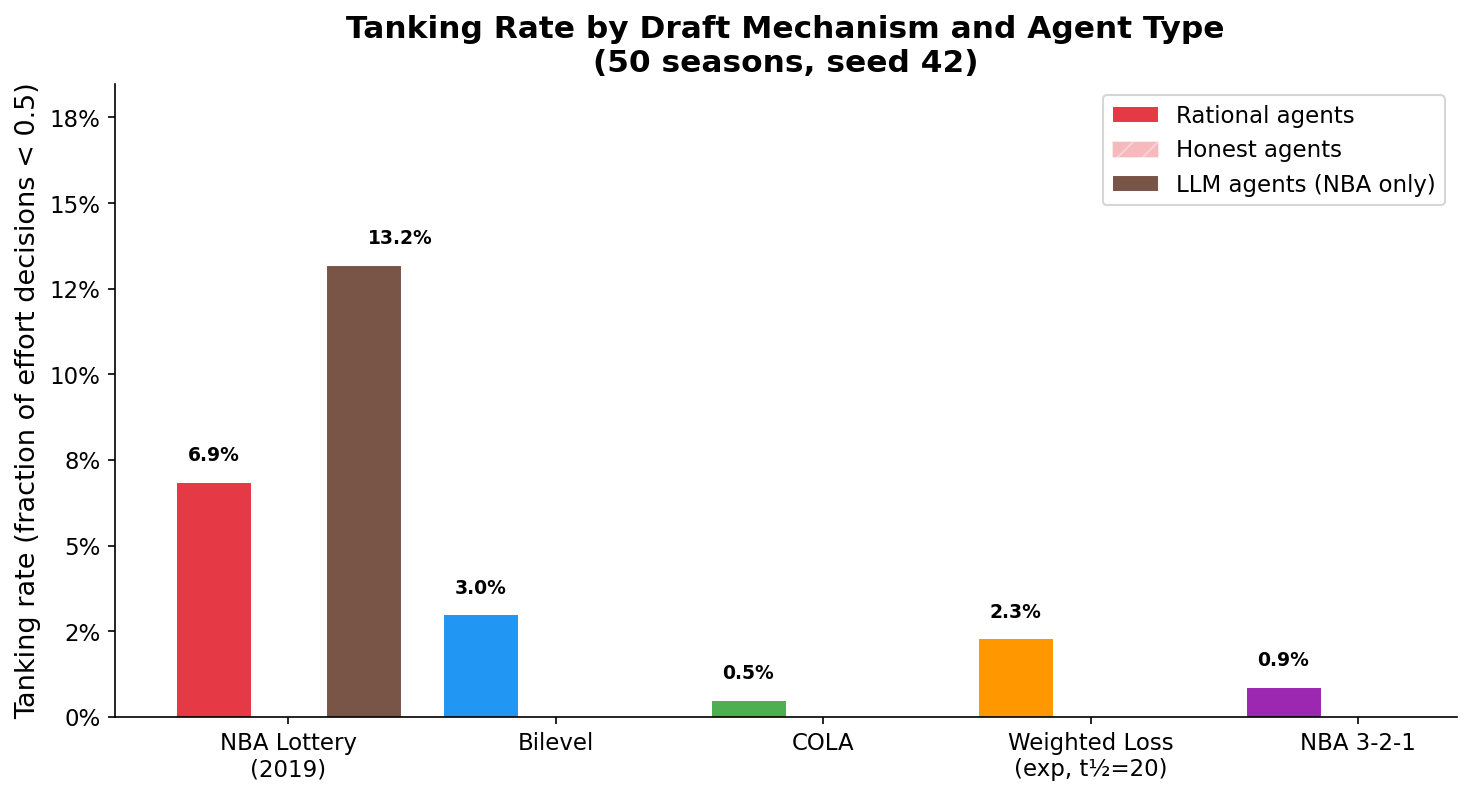
\includegraphics[width=0.85\textwidth]{figures/fig1_tanking_by_mechanism.png}
\caption{Mean tanking rate (fraction of decisions with $e < 0.5$) for each
mechanism under all-rational agents, averaged over 50 seasons.
Error bars show one standard deviation across seasons.
The current NBA lottery produces the highest rate (6.9\%); COLA and NBA 3-2-1
achieve the lowest.}
\label{fig:tanking}
\end{figure}

\begin{figure}[h]
\centering
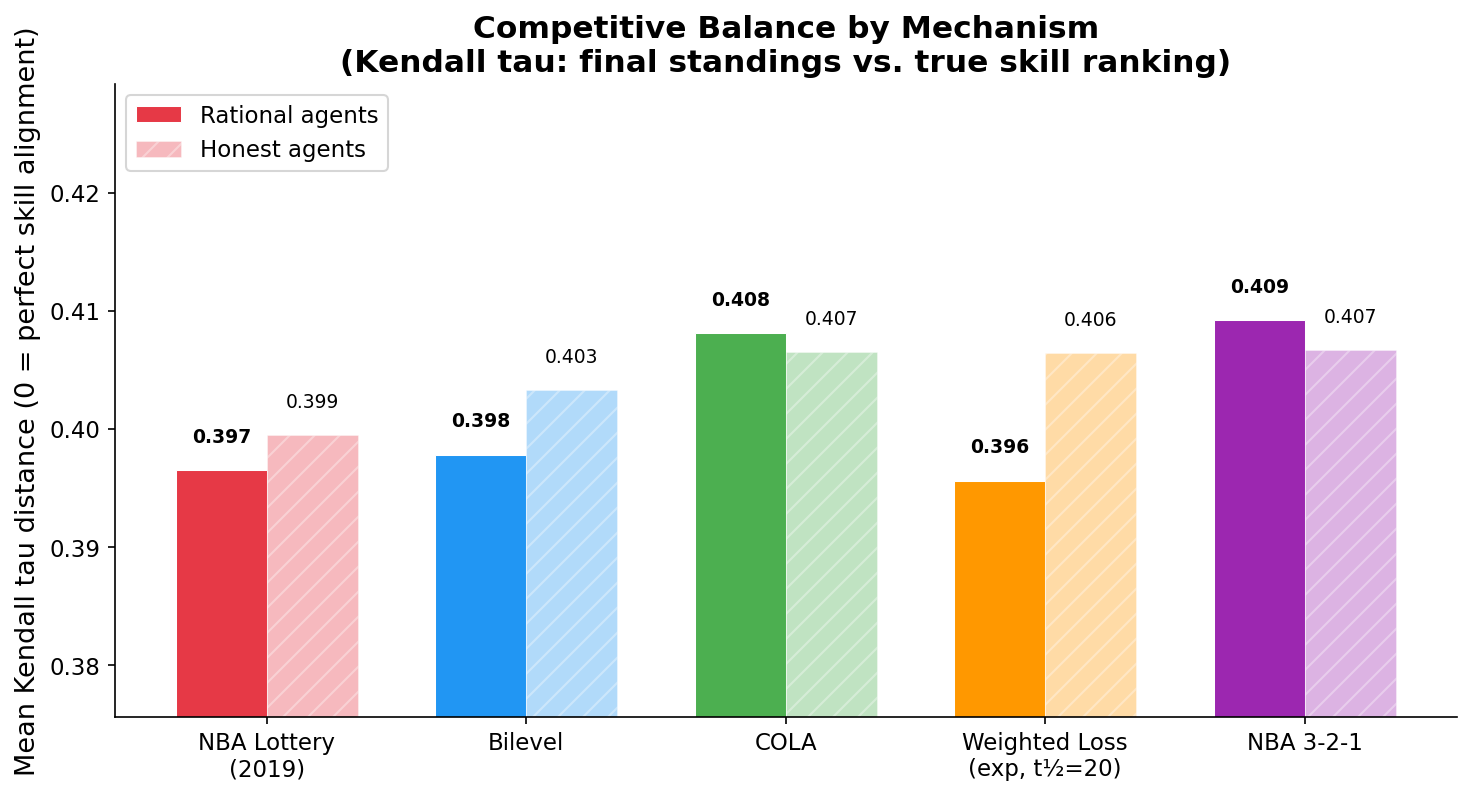
\includegraphics[width=0.85\textwidth]{figures/fig2_tau_by_mechanism.png}
\caption{Mean Kendall tau distance between final standings and true skill
ranking, for rational agents (blue) and honest agents (orange).
Tau measures how well the draft's redistributive mechanism tracks actual team
quality; lower is better.
Differences across mechanisms are small, reflecting that with $V=200$ most
teams compete seriously, limiting strategic distortion of standings.}
\label{fig:tau}
\end{figure}

\begin{figure}[h]
\centering
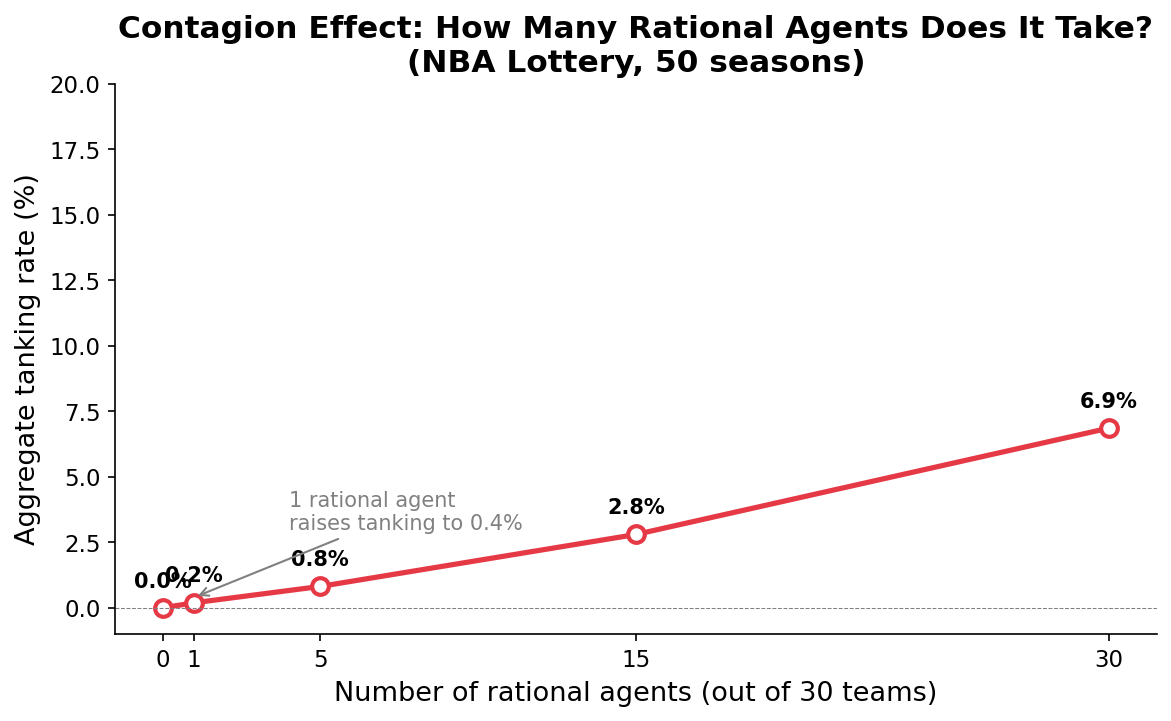
\includegraphics[width=0.75\textwidth]{figures/fig3_mixed_sweep.png}
\caption{Mixed-population sweep: aggregate tanking rate as the number of
rational agents increases from 0 to 30 under the current NBA lottery.
The relationship is approximately linear with no evidence of a strategic
tipping point.}
\label{fig:mixed}
\end{figure}

\begin{figure}[h]
\centering
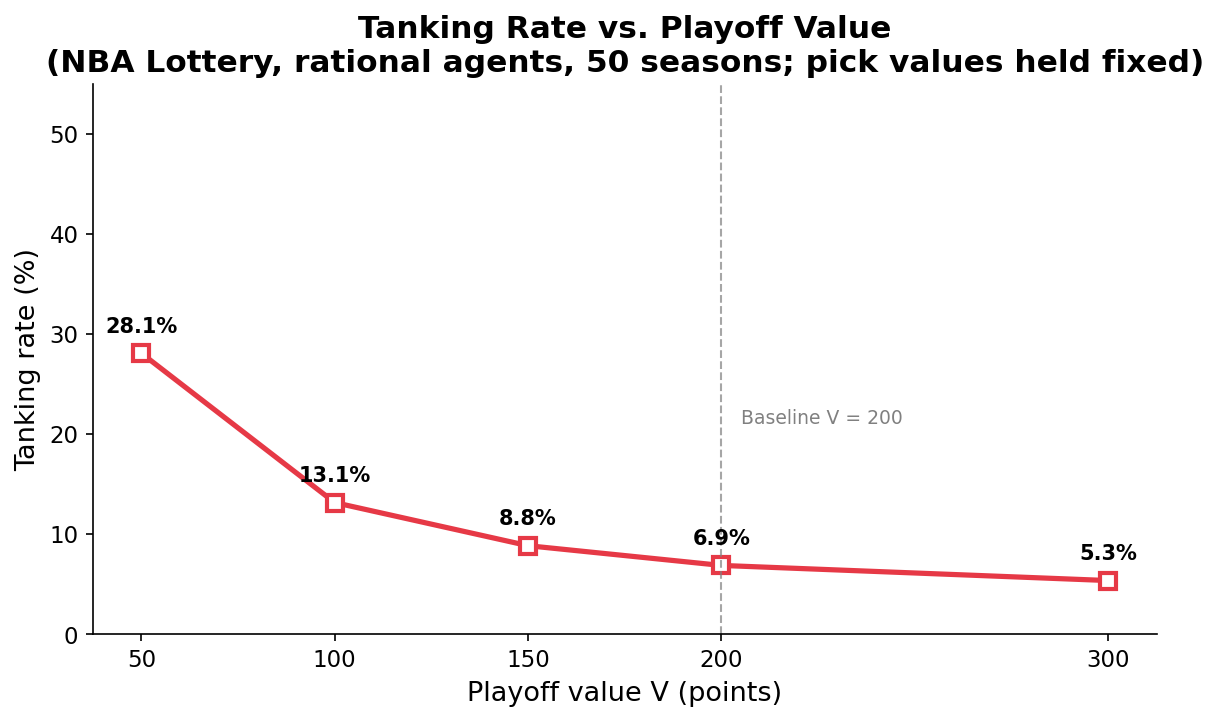
\includegraphics[width=0.75\textwidth]{figures/fig4_playoff_value_sweep.png}
\caption{Playoff-value sensitivity sweep: tanking rate under the NBA lottery
as $V$ varies from 50 to 300.
The decline is continuous and monotone, reflecting the probabilistic
expected-utility model.
At $V=200$ (baseline), tanking is concentrated among teams with negligible
playoff probability rather than bubble teams.}
\label{fig:pvsweep}
\end{figure}

\begin{figure}[h]
\centering
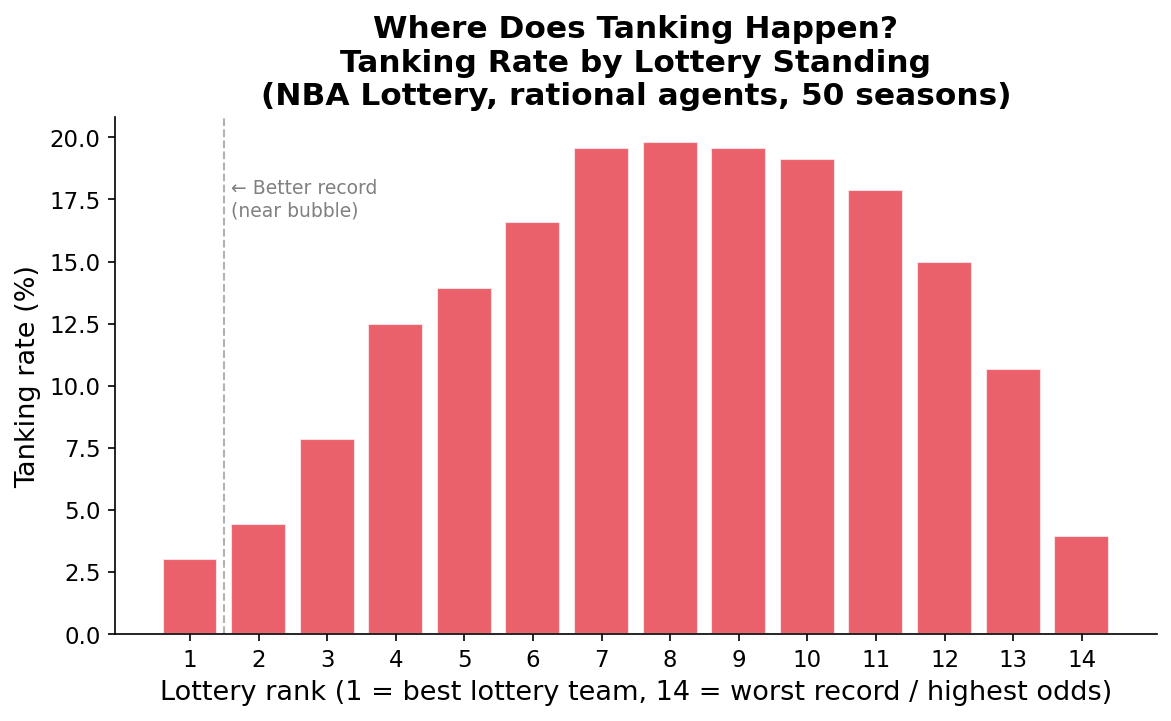
\includegraphics[width=0.75\textwidth]{figures/fig6_tanking_by_lottery_rank.png}
\caption{Tanking decisions by team lottery rank (1 = worst record) under the
NBA lottery with all-rational agents.
The incentive is concentrated in lottery ranks 5--11, confirming Conjecture~2:
with high playoff value, the tanking incentive is sharpest in the middle of
the lottery tier, not at the absolute bottom.}
\label{fig:byrank}
\end{figure}

\begin{figure}[h]
\centering
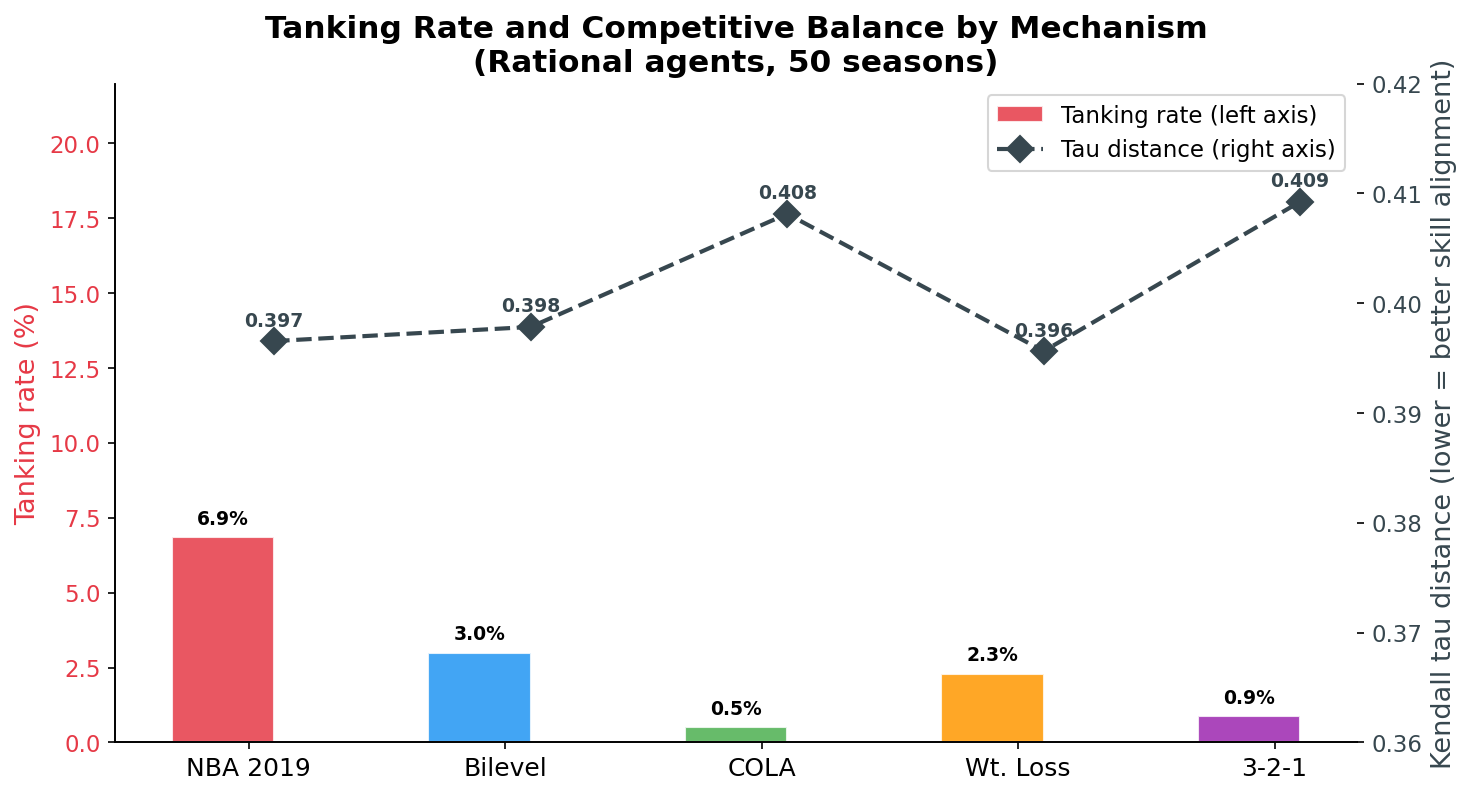
\includegraphics[width=0.85\textwidth]{figures/fig7_summary_dual_axis.png}
\caption{Summary comparison of all five mechanisms: tanking rate (left axis,
bars) and draft efficiency for the weakest quartile (right axis, markers).
Lower tanking and lower mean pick number are both desirable.
NBA 3-2-1 achieves the best draft efficiency (6.57) while maintaining low
tanking (0.9\%).}
\label{fig:summary}
\end{figure}

\section{NBA Draft Lottery Odds Under Each Mechanism}
\label{app:odds}

\begin{table}[h]
\centering
\renewcommand{\arraystretch}{1.2}
\begin{tabular}{r r r r r r}
\toprule
\textbf{Rank} & \textbf{NBA 2019} & \textbf{Bilevel} & \textbf{COLA}
              & \textbf{Wt.\ loss} & \textbf{3-2-1} \\
\midrule
1  & 14.0\% & 14.0\% & 7.1\% & order-dep.\ & 5.9\% \\
2  & 14.0\% & 14.0\% & 7.1\% & order-dep.\ & 5.9\% \\
3  & 14.0\% & 14.0\% & 7.1\% & order-dep.\ & 5.9\% \\
4  & 12.5\% & 12.5\% & 7.1\% & order-dep.\ & 8.8\% \\
5  & 10.5\% & 10.5\% & 7.1\% & order-dep.\ & 8.8\% \\
6  &  9.0\% &  9.0\% & 7.1\% & order-dep.\ & 8.8\% \\
7  &  7.5\% &  7.5\% & 7.1\% & order-dep.\ & 8.8\% \\
8  &  6.0\% &  6.0\% & 7.1\% & order-dep.\ & 8.8\% \\
9  &  4.5\% &  4.5\% & 7.1\% & order-dep.\ & 8.8\% \\
10 &  3.0\% &  3.0\% & 7.1\% & order-dep.\ & 8.8\% \\
11 &  2.0\% &  2.0\% & 7.1\% & order-dep.\ & 8.8\% \\
12 &  1.5\% &  1.5\% & 7.1\% & order-dep.\ & 8.8\% \\
13 &  1.0\% &  1.0\% & 7.1\% & order-dep.\ & 8.8\% \\
14 &  0.5\% &  0.5\% & 7.1\% & order-dep.\ & 8.8\% \\
\bottomrule
\end{tabular}
\caption{Approximate probability of winning the \#1 pick under each
mechanism by lottery rank (1 = worst record). COLA gives equal odds to all
lottery teams. Weighted loss depends on the team's cumulative loss score, not
its rank, so exact odds are trajectory-dependent. For the NBA 3-2-1 proposal,
Tier~A (ranks 1--3) receive 2 balls and Tier~B (ranks 4--14) receive 3 balls,
out of a pool of $3 \cdot 2 + 11 \cdot 3 = 39$ total balls.
Picks 1 through 14 are all drawn sequentially from the weighted pool.}
\label{tab:odds}
\end{table}

\section{Individual Paper Summaries}
\label{app:paper_summaries}

\subsection{\citet{banchio2020}: ``A No-Tanking Draft Allocation Policy''}

\textbf{In one sentence:} This paper identifies that since any end-of-year
ranking system will create perverse incentives, the NBA should only account
for games up to the point at which a team first has an incentive to tank.

\subsubsection*{Setting \& Model}
\begin{itemize}
    \item Teams are the agents, each choosing an effort level that affects
    their probability of winning individual games and, ultimately, their
    end-of-season rank.
    \item The season is modeled as a sequence of pairwise games; team effort
    translates to win probability through a parameter $\alpha$.
    \item The league is modeled as a central planner whose objective is to
    maximize the probability that the first draft pick is assigned to the
    worst team, subject to the constraint that no team has an incentive to
    tank at any point in the season.
    \item The proposed mechanism updates lottery probabilities dynamically
    after each game, setting each team's probability to match its current
    likelihood of finishing last given the season history so far.
    \item This adjustment process is terminated before continuing it would
    violate incentive-compatibility for any team: the cutoff is endogenous to
    the season's trajectory, not fixed in advance.
\end{itemize}

\subsubsection*{Main Results}
\begin{itemize}
    \item \textbf{Impossibility (Theorem 1):} Any redistributive policy that
    relies on final standings alone to allocate draft picks will give some team
    an incentive to lose in some possible season history. Proved by
    contradiction.
    \item \textbf{Positive result:} Their dynamic mechanism sidesteps the
    impossibility by locking in lottery probabilities mid-season, before
    tanking becomes rational. It is approximately optimal among all
    incentive-compatible rules that operate on the same restricted set of games.
    \item The mechanism does not guarantee the best player goes to the worst
    team, but approximates it far better than a flat uniform lottery would.
\end{itemize}

\subsubsection*{Proof Techniques / Methodology}
\begin{itemize}
    \item Theorem 1: proof by contradiction.
    \item Simulation of a single season at a time to identify the cutoff point.
    \item Retroactively applied to the 1987 and 1989 NBA seasons: flat lottery
    odds in those seasons means the data is not contaminated by teams already
    behaving strategically.
\end{itemize}

\subsubsection*{Relation to Our Project}
\begin{itemize}
    \item Their model setup is very robust; we implement a simplified version.
    \item We adopt their framework for a value from the draft $D$ and a value
    from making the playoffs $V$.
    \item We do not use their $\alpha$ parameter for effort; instead we use an
    effort floor model in which teams cannot perfectly throw a game even at
    minimum effort.
\end{itemize}

\subsubsection*{Critiques / Open Questions}
\begin{itemize}
    \item To calculate when draft odds should be locked in, the league must
    know both $D$ and $V$ for each team; in practice these are unobservable
    and likely heterogeneous across franchises.
    \item The game at which draft order is set is not transparent or
    predictable in advance, which creates fan engagement and trust problems.
    \item Ignores game outcomes from the latter part of the season entirely,
    which may reduce competitive effort even absent intentional tanking.
    \item No incentive for teams to continue playing hard after the cutoff
    point is reached.
\end{itemize}

\subsection{\citet{kazachkov2020}: ``On Tanking and Competitive Balance''}

\textbf{In one sentence:} This paper introduces a bilevel ranking mechanism
that determines non-playoff draft order by standings at a mid-season
breakpoint rather than end of season, proving it both reduces tanking and can
improve competitive balance relative to the current NBA system.

\subsubsection*{Main Results}
\begin{itemize}
    \item Under the current NBA system, tanking is a dominant strategy for
    any team effectively eliminated from playoff contention.
    \item Under the bilevel mechanism, no team has an incentive to tank in any
    game after the breakpoint has passed.
    \item Simulation results show the bilevel ranking reduces tanked games by
    57--72\% compared to the current NBA system, depending on breakpoint
    placement.
    \item The optimal breakpoint falls between 5/6 and 7/8 of the way through
    the season.
    \item We borrow their Kendall tau distance metric as our primary measure
    of competitive balance.
\end{itemize}

\subsubsection*{Critiques / Open Questions}
\begin{itemize}
    \item The breakpoint must be chosen in advance; no principled method is
    provided for determining the optimal breakpoint.
    \item Teams could tank strategically before the breakpoint to position
    themselves favorably.
    \item Their simulations use rule-based agents with fixed strategies; our
    simulation directly addresses this limitation.
\end{itemize}

\subsection{\citet{highley2026}: ``Carry-Over Lottery Allocation''}

\textbf{In one sentence:} COLA achieves full incentive compatibility by giving
every non-playoff team the same number of lottery tickets each season
regardless of record, while still favoring persistently weak teams through
ticket carryover across seasons.

\subsubsection*{Main Results}
\begin{itemize}
    \item Classic COLA eliminates the in-season tanking incentive entirely:
    ticket allocation does not depend on record.
    \item The carryover structure preserves the competitive balance function
    of the draft; teams that repeatedly miss the playoffs accumulate more
    tickets over time.
    \item Diet COLA is formally proved incentive-compatible under the
    assumption that reaching the playoffs is always preferred to lottery access.
    \item The Bayesian Truth Serum mechanism for identifying strong draft
    classes is a notable methodological contribution.
\end{itemize}

\subsubsection*{Critiques / Open Questions}
\begin{itemize}
    \item Multi-year ticket carryover introduces significant administrative
    complexity.
    \item The Bayesian Truth Serum mechanism may itself be manipulable if
    media respondents have team affiliations or financial incentives.
    \item The IC proof depends on the assumption that all teams always prefer
    playoff access to lottery access; if this fails more broadly, the IC
    guarantee weakens.
\end{itemize}

\subsection{\citet{taylor2002}: ``Losing to Win''}

\textbf{In one sentence:} An early empirical paper that quantified tanking
by exploiting two lottery-regime changes to show that eliminated teams' win
rates correlate strongly with the incentive structure of the active lottery.

\subsubsection*{Main Results}
\begin{itemize}
    \item 1983--84: eliminated teams $2.5\times$ as likely to lose vs.\
    expected from team quality.
    \item 1984--85 (flat odds): effect drops to $1.3\times$.
    \item 1990 (weighted odds restored): $2.2\times$.
    \item Lottery structure significantly impacts the propensity of eliminated
    teams to lose.
\end{itemize}

\subsection{\citet{schmidt2024}: ``On the Incentive Structure of Tournaments''}

\textbf{In one sentence:} Uses modern portfolio theory to show that the NBA's
2019 flattening of top-pick odds led to a measurable decline in asset
deployment quality among lottery-contending teams, with effects disappearing
after the reform.

\subsubsection*{Main Results}
\begin{itemize}
    \item 2017--18: lottery-contending teams measurably underdeployed their
    best lineups relative to a theoretically optimal frontier.
    \item 2018--19: effect disappears after odds are flattened.
    \item Road games show a larger tanking effect than home games.
\end{itemize}

\subsection{\citet{lenten2016}: ``Mitigation of Perverse Incentives in
Professional Sports Leagues''}

\textbf{In one sentence:} Proposes assigning draft picks by order of playoff
elimination, arguing this locks in draft position before teams have incentive
to lose.

\subsubsection*{Main Results and Critique}
\begin{itemize}
    \item Controlling for other factors, teams play meaningfully better in
    the post-elimination window than the pre-elimination window.
    \item \citet{banchio2020} counter that this pushes the tanking incentive
    earlier in the season rather than eliminating it, creating a race to
    elimination rather than a race to the bottom.
\end{itemize}

\end{document}